%  chapter-04.tex

\chapter{Implementation}

In this chapter we describe our specific implementation of the design described in Chapter 3. For many of the components in our implementation we either use directly or modify existing open source components. We truly are standing on the shoulders of giants\cite{ben-yehuda_osr_2008}. We make some implementation choices based on the software technologies available, including our tendency to prefer open source and open standards-based technologies. We successfully deployed our Rapid Recovery Desktop system on a wide variety of hardware. 

In terms of virtualization we made use of the libvirt toolkit\cite{libvirt_website}, which can be used to interact with a variety of virtualization systems. Next, we define a basic virtual machine contract system and describe how it is integrated with our own virtualization security framework. Then, we show our implementation of two key enforcement elements, an FS-VM and NET-VM. Finally, pulling it altogether, we show some example virtual appliances that we have created. 

\section{Virtualization Components}

\subsection{Virtualization Types}
There are many different types of virtualization options. A common breakdown is into the categories of emulation, full, para, operating system level, library, application. Emulation is when a different architecture is being created (virtualized) often in order to simulate hardware that is not available (for example, some legacy applications require old hardware) or for development on new platforms that hardware is still being developed (for example, mobile platform emulators). Emulators typically run much slower than other types of virtulization, since all of the virtualization/emulation is done is software.

Full virtualization is creating a virtualized version of the same platform (for example, x86 on x86). Full virtualization is one of the most common types of virtualization. It performs relatively well, since most of (or sometimes all of) the operation can be performed on platform being virtualized. We rely on hardware support for virtualization in order to provide full virtualization support on Xen and KVM.

Paravirtualization is when the guest operating system kernel is modified in order to support virtualization. The virtualized platform is the same and the performance of this type of virtualization is fast, since the guest is able to be made virtualization-aware.  The limitation to this type of virtualization is that the operating system kernel source must be available. We use this type of virtualization for open source operating systems running on Xen.

Operating System level virtualization (also commonly referred to as container-based), is when the virtual guests share the kernel of the host system. This is a very fast option, but limits the guest type to be the same as the base system (for example, Linux guests must run on a Linux base). Also, providing performance isolation (one guest consuming lots of resources not affected other guests) has traditionally been difficult to implement with operating system level virtualization. 

The last two types of virtualization, library and application that we mention are not used to virtualize operating system instances, but instead run at the application layer. Library virtualization is typically done to emulate an operating system or subsystem (for example, Wine provides a subset of the Win32 API to allows Windows applications to run on Linux). Finally, application virtualization provides a managed runtime environment in order to have cross platform application mobility (for example, the Java runtime environment).

\subsection{Hypervisor Component}

As described in our design, we aim to provide isolation and the ability to run multiple different operation systems efficiently, so we choose to focus our initial implementation on full virtualization and paravirtualization. However, since there are many different types of virtualization that we could have used to demonstrate the feasibility of our approach.  We chose to make use of the open source virtualization toolkit libvirt, which has support to interact with Xen, QEMU, KVM, LXC, OpenVZ, User Mode Linux, VirtualBox, and VMware GSX and ESX\cite{libvirt_website}. Integrating support for libvirt allows users to easily switch to different virtualization solutions to meet their particular needs.

The performance, isolation, and other properties of the various types of virtualization systems has been well studied, in particular we did a isolation performance comparison of various virtualization systems in\cite{isolation_paper_2007}. Container-based (OS-level virtualization) solutions, such as LXC and OpenVZ, that use a shared system kernel tend to provide better scalability and performance, but with the trade-off of weaker isolation properties. Container-based solutions are also limited to being able to only run a single type of guest operating system (for example, Linux on Linux).  On the other hand, platform virtualization systems, such as Xen or KVM, are able to provided stronger isolation properties and can run a variety of operating system guests (for example, Linux and Windows guests). Since we are willing to trade off some performance for isolation properties (for security reasons) and the added flexibility of being able to support heterogeneous guest operating systems, for our initial implementation we choose to support the two leading open source platform virtualization systems, specifically, the stand-alone Xen hypervisor and the integrated Linux/KVM hypervisor. However, adding support for other virtualization systems, especially, but not limited to, those supported by libvirt, should be straight forward.

Xen and KVM take different approaches to the implementating a hypervisor. Xen uses a stand-alone hypervisor and separate management domain, while KVM takes a integrated hypervisor approach by integrating into Linux. Our architecture is flexible enough to work with both of these approaches as depicted in Figures \ref{fig:IntegratedHypervisor} and \ref{fig:StandAloneHypervisor}. Figure \ref{fig:IntegratedHypervisor} depicts our architecture integrated with the Linux/KVM hypervisor. Note that OSCKAR is installed in the management domain. For the Linux/KVM case, the hypervisor is placed at the same privilege level as the management domain, which does not impact our threat model. The only minor limitation of the current KVM approach is that running a true driver domain (when a guest gets full access to device and provides virtual device access to other guests) would be challenging\cite{kvm_driver_domain_2009}. This would mean that adding the performance and security benefits of using an IOMMU (as discussed in related work) for the FS-VM or NET-VM would require some implementation effort on KVM.

\begin{figure}[tbp]
\begin{centering}
\rotcaption{Our Achitecture on a Integrated Hypervisor}
\label{fig:IntegratedHypervisor}
\includegraphics[scale=0.7,angle=90]{figs/IntegratedHypervisorArchitecture}
\end{centering}
\end{figure}

Figure \ref{fig:StandAloneHypervisor} depicts our architecture integrated with the Xen Hypervisor. The main difference between these two configurations is the placement of the hypervisor. The hypervisor is placed at a higher privilege level in the Xen case and at the same privilege level in the Linux/KVM case. OSCKAR is also installed in the management domain in the Xen case. The advantage of using Xen is the ability to make use of a driver domain for the FS-VM or NET-VM with an IOMMU without extra implementation work as would be needed with KVM.

\begin{figure}[tbp]
\begin{centering}
\rotcaption{Our Achitecture on a Stand-alone Hypervisor}
\label{fig:StandAloneHypervisor}
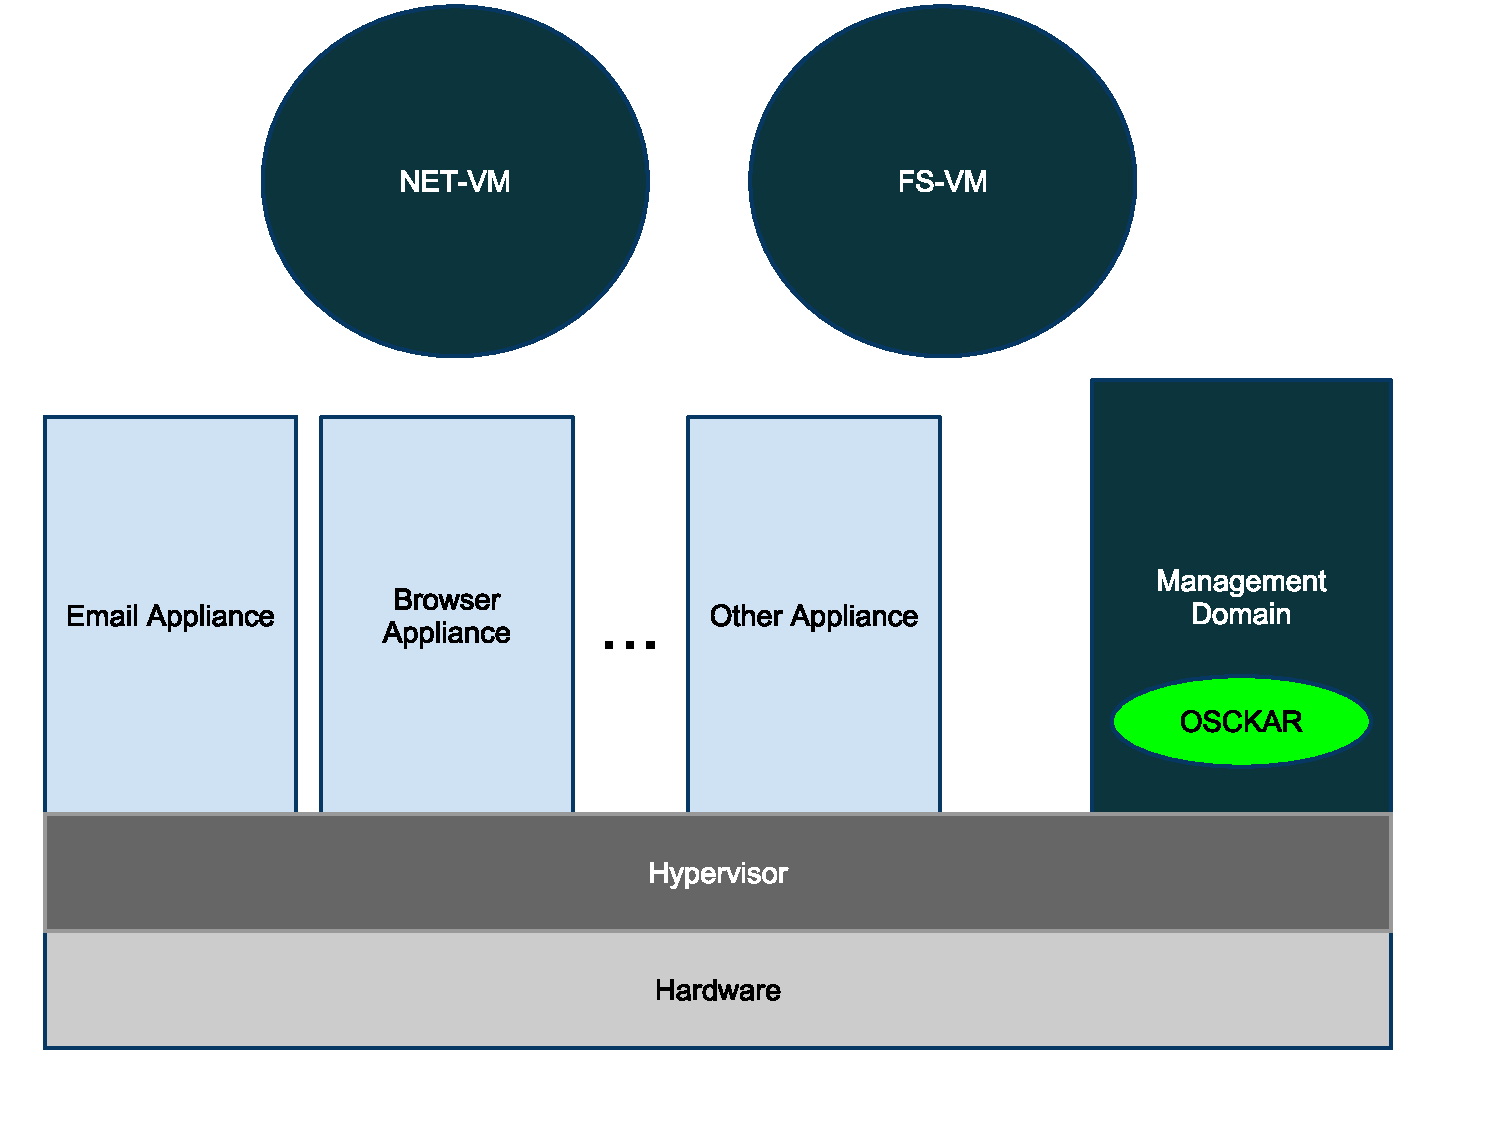
\includegraphics[scale=0.7,angle=90]{figs/StandAloneHypervisorArchitecture}
\end{centering}
\end{figure}

Some of the differences between the stand-alone and integrated hypervisor approaches are analogous to the inherent differences between micro kernels and monolithic kernels in the operating system space. For instance, having a standalone hypervisor can allow for separation or dissagregation\cite{murray_2008}, but this approach may require more communication overhead in order for the various components to communicate. On the other hand, having an integrated hypervisor may allow for tight communication and sharing of functionality among the hypervisor and management domain, but may lead to less isolation of components, which in turn could cause a single component to negatively affect the system, more than if it had been separated out, as could be done in the standalone hypervisor case.

From a practical standpoint, the integrated hypervisor approach allows for installing and loading the hypervisor without requiring a reboot, while the standalone hypervisor needs the system to be restarted, so that the the hypervisor is the first to be loaded on the hardware, and therefore more privileged. This minor difference alone is not reason enough to choose an integrated hypervisor over a stand-alone hypervisor, but is just one example of minor differences that exist between the two hypervisor approaches. Further discussion of the differences between stand-alone and integrated hypervisors is outside the scope of this dissertation, but the curious reader can explore some of the related papers and articles on this topic, such as ~\cite{kvm_ols07, clark_2004, kvm_vs_xen_at_xen_summit_2008, redhat_rhel_54_2009, crosby_xen_dead_2008, cnet_hypervisor_2010, crosby_novell_2010, liguori_truth_2008,rhev_2009,qubes-os_2010}. We conclude our discussion by noting that our design is able to effectively support either of the hypervisor configurations to allow the users to make use of different solutions as they may need or want to.

\subsection{VMM Interface}
\label{sec:vmm-implementation}


In chapter 3, we described our design of OSCKAR and its inclusion of a VMM interface. The VMM interface that we integrated into our Rapid Recovery Desktop implementation provides a high level interface to manage virtual machines. With our VMM interface, virtual appliances, which are just special virtual machines, can use libvirt or directly use the underlying virtualization technologies, such as Xen or KVM. In this way, our VMM interface allows for both the generic use of libvirt-based VMs (a generic vmm ruleset type) and also for the specific use of features provided by the various virtualization systems (specific vmm ruleset types). This allows users who is familar with libvirt-based VMs to use them and also for users that are familar with a particular system to use it. This type of support is also important since libvirt may implement a specific feature in a way that is convenient for the user or libvirt may not have yet implemented a specific feature that exists in a specific system. Our VMM interface lets users be able to use either a libvirt backend, the default, or choose a specific backend, such as Xen or KVM, as needed. 

Some example VMM rulesets are shown in Figure \ref{lst:generic-vmm} and \ref{lst:specific-vmm}. In Figure \ref{lst:generic-vmm}, the ruleset type is set to vmm and in Figure \ref{lst:specific-vmm} the ruleset is set to qemu-spice.  Note that rulesets are only a subset of the full contract). We will build up various rule set throughout the chapter and tie them together with a full virtual appliance and virtual machine contract (VMC) example at the end of the chapter.

In the vmm ruleset case (Figure \ref{lst:generic-vmm}), the virtual appliance designer is letting the VMM interface decide what virtualization software to use. For this case, our VMM interface uses libvirt, which would mean that we could run on a variety of virtualization systems (we simply need to detect what is available and configure accordingly). In the qemu-spice case (listing \ref{lst:specific-vmm}), the virtual appliance designer is specifying that qemu-spice is used as the hypervisor. This is required since the Spice VDI system, which is a virtual desktop infrastructure system, is currently only available in a special version of QEMU\footnote{Spice support is expected to be in upstream QEMU soon, see: http://spice-space.org/page/Features/QemuIntegration} and so the appliance designer needs to specify that hypervisor, so that he knows the options related to Spice are available.

The rest of the options in the figures specify memory, disk, network, and other features. Our VMM interface converts these high level options to the appropriate backend (libvirt, Xen, KVM, etc.). The only coordination needed is between the VMM interface designer and the virtual appliance designer. The VMM interface designer needs to make the allowed options and XML syntax available. The implementation details are not needed by the appliance designer. This structure allows the specific design details to be left to the interface designers. In this specific case, we implemented the VMM interface ourselves to meet our needs, but another VMM interface could be implemented that works very differently. For example, there could just as easily be a proprietary VMM interface component that published the high level XML interface that it supports. Similarly, a VMM interface designer could add rules to specify more advanced security policies at the VMM layer. 

We described in Chapter 3 the concept of interfaces registering for events and then responding to signalling. In this specific case, our VMM interface registers for events of the form vmm.* and qemu-spice.* events (for example, vmm.start\_vm and qemu-spice.start\_vm). Then, when the virtual appliance is added to the system the Policy Manager sends the appropriate ruleset block to our VMM interface. The VMM interface then configures a VM as appropriate and is able to manage it (start, stop, etc.) as needed. The VMM interface designer does not necessarily need to know anything about virtual appliances at all, but only how to manager VMs. The higher level control components, such as a Rapid Recovery Desktop control component makes the calls to the appropriate interfaces to handle the high level logic of our system.

\begin{figure}[tbp]
\caption{VMM rule set that uses the generic vmm backend chosen by the VMM interface}
\label{lst:generic-vmm}

\begin{lstlisting}
 <ruleset type="vmm">
    <name>browser</name>
    <memory>
      <min>128MB</min>
      <max>1G</max>
      <default>512MB</default>
    </memory>
    <disks>
      <cowdisk type="qcow2" cowbase="browser.qcow2">browser</cowdisk>
    </disks>
    <vnics>
      <vnic type="bridge" />
    </vnics>
    <graphics>
      <graphic type="vnc" />
    </graphics>
    <displays>  
      <display type='vga' />
    </displays>
    <features>
      <feature>acpi</feature>
    </features>
  </ruleset>
\end{lstlisting}
\end{figure}

\begin{figure}[tbp]
\caption{VMM rule set that uses the specific qemu-spice backend}
\label{lst:specific-vmm}

\begin{lstlisting}
<ruleset type="qemu-spice">
    <name>browser</name>
    <memory>
      <min>128MB</min>
      <max>1G</max>
      <default>512MB</default>
    </memory>
    <disks>
      <cowdisk type="qcow2" cowbase="browser.qcow2">browser</cowdisk>
    </disks>
    <vnics>
      <vnic type="bridge" />
    </vnics>
    <graphics>
      <graphic type='spice' port='5930' />
    </graphics>
    <displays>  
      <display type="qxl" />
    </displays>
    <features>
      <feature>acpi</feature>
    </features>
  </ruleset>
\end{lstlisting}
\end{figure}

\subsection{Builder Interface}
\label{sec:builder-implementation}

Another key component of the virtualization interface is a virtual machine builder interface. In order for users or virtual appliances designers to create new virtual appliances, they need a mechanism to do so. We provide a builder interface, which we have implemented as a stand-alone component, but is a component that we may integrate into our VMM interface in the future. The builder interface allows users to use a contract to specify what type of guest needs to be built and other disk parameters (size of disk, file system type, copy on write support, etc.). An example contract is shown in Figure \ref{lst:builder-ruleset}. The builder contracts specify the basic properties of the virtual appliance images, such as operating system type, the disk partitioning scheme, users, and packages to include.

Our current builder implementation only supports building Ubuntu images, since we are using the Virtual Machine Builder (vmbuilder)\cite{vmbuilder_website} developed for Ubuntu. Similarly, we could support of Linux distributions by integrating support for a tool like Stacklet\cite{stacklet_website}, which is able create a wide variety of Linux images. We could also support CD-based installs of operating systems such as Windows, which VMware, Microsoft, and others have made some tools that can automate much, or all, of the process, similar to how Linux or Unix-based installations can be automated. Integration of such components is an interesting area of future implementation work.

Even without an automated process, manual creation of virtual machine disk images can be made. For example, an existing installation can be converted into a virtual disk installation. Also, manual creation of virtual disk images can be as easy as installing manually from installation media, such as a CD or DVD, or by simply populating a virtual disk image with the files needed to boot and run an operating system\cite{runningxen_book}.

As a future extension to our builder interface, we could automate the process of adding the mount points needed by the FS-VM and various other enforcement elements that may be needed.

\begin{figure}[tbp]
\caption{Builder rule set}
\label{lst:builder-ruleset}

\begin{lstlisting}
 <ruleset type="builder">
    <os type="linux" flavor="ubuntu" version="9.10" />
    <disk type="disk" size="10240" sparse="true" format="qcow2">
       browser.qcow2</disk>

    <partitions>
      <partition filesystem="ext3" mountpoint="/" size="10G" 
         bootable="true">1</partition>
    </partitions>

    <users>
      <user logindisabled="true">root</user>
      <user password="ubuntu" groups="ubuntu,admin">
         ubuntu</user>
    </users>
    
    <packages>
      <package name="openssh-server" action="add" />
      <package name="sl" action="add" />    
    </packages>

    <installmirror>http://mirror.clarkson.edu/ubuntu</installmirror>
 </ruleset>
\end{lstlisting}
\end{figure}

\section{OSCKAR}

We needed to create and maintain a highly extensible and highly useful security policy
enforcement framework and API to enable product developers, such as developers of the Rapid Recovery Desktop product, to easily create practical, high-quality products that respond to real-world problems. So, we created the OSCKAR virtualization security framework. OSCKAR is a Python library, implemented with an Event Chat message bus and Policy Manager security daemon as described in Chapter 3. 

Event Chat is currently implemented in python as a multi-threaded TCP socket server and request handler (SocketServer.ThreadingTCPServer and SocketServer.BaseRequestHandler in Python 2 (SocketServer has been renamed socketserver in Python 3.0)). Event Chat currently supports the process of an enforcement element registering for events and the process of signalling an event. An Event Chat reply mechanism is currently being developed, which will improve error handling and efficiency of message passing.

Even though Event Chat lacks a reply mechanism, it is stable and robust enough to meet our current needs. The reply mechanism will likely make implementation of various interfaces easier. The reply mechanism is also the last bit of core functionality that Event Chat should need, since it is only a message passing bus. The fact that enforcement elements can register for events that they can handle and then be signaled to respond to the various events that they are registered for means that any number of enforcement elements can be created and added to the system to handle events raised. Event Chat by design does not perform any other actions. It is just a communication mechanism. Other mechanisms, such as restful servers\cite{restful_phdthesis} or remote procedure call (RPC) servers could easily provide the same functionality. These types of design and implementation alternatives are outside the scope of this dissertation, but could be an interesting area of future exploration.

The policy and actions that are taken are delegated to Policy Manager. Our Policy Manager component is implemented in python and is a simple TCP socket client that connects to Event Chat and, based on contracts, responds to and raises the appropriate events. Policy Manager can be configured to run almost exclusively based on contract policy, since operation logic can be coded into both global policy contracts and virtual machine contracts. There is a global policy contract and one or more local contracts for the various virtual appliances. An administrator can configure, in a global policy file, that zero or more events are raised in response to a given event. For example, on a ``START\_VM'' event, policy manager is configured to send the appropriate contracts to the appropriate enforcement elements and raise the appropriate event to the VMM interface to start the VM. 

Figure \ref{lst:PolicyManager_global} shows an example global Policy Manager contract. The basic idea is that there are a set of events that are handled by raising the appropriate events. When a new virtual appliance is added to the system, the first step is to send its VMC to Policy Manager. This is accomplished by raising an IMPORT\_VMC event and passing the contract as the argument (\$ARG in the contract, which is replaced with the actual contract passed during the at runtime). To start that virtual appliance, a START\_VM event needs to be passed, with the unique VM name or ID as argument. Policy manager will then send the rule sets to the appropriate enforcement elements. The enforcement elements then set up the environment to support the VM (for example, the VMM interface creates the config file and the NET-VM sets up the network(s)) Then, if all the enforcement elements are in place and return success, Policy Manger can then send an event to the VMM interface to start the VM. 

\begin{figure}[tbp]
\caption{A Sample Policy Manager Global Contract. Note that the \$ARG is simply the argument to the event. \$ARG is replaced with the argument passed during the event at runtime}
\label{lst:PolicyManager_global}

\begin{lstlisting}
<contract type="global_PolicyManager_policy">
  <ruleset type="response">
    <handle event="IMPORT_VMC">
      <raise event="PolicyManager.import_contract" argument="$ARG " />
    </handle>
    <handle event="START_VM">
      <raise event="PolicyManager.send_subcontracts" argument="$ARG" />
      <raise event="vmm.start_vm" argument="$ARG" />
    </handle>
  </ruleset>
</contract>
\end{lstlisting}
\end{figure}


A high-level diagram of this process is depicted in Figure \ref{fig:StartVM}. In step 1, a control element sends a complete VMC into the system through Event Chat with an IMPORT\_VMC event. In step 2, the VMC is communicated to Policy Manager. In step 3, Policy Manager sends the relevant portions of the contracts (subcontracts) to the enforcement elements (FS-VM and NET-VM) and the core component (VMM interface). In step 4, the enforcement elements and core components respond with an OK. In step 5, a START\_VM event is issued.

\begin{figure}[tbp]
\begin{centering}
\caption{Process of importing virtual machine contract (VMC) and starting VM}
\label{fig:StartVM}
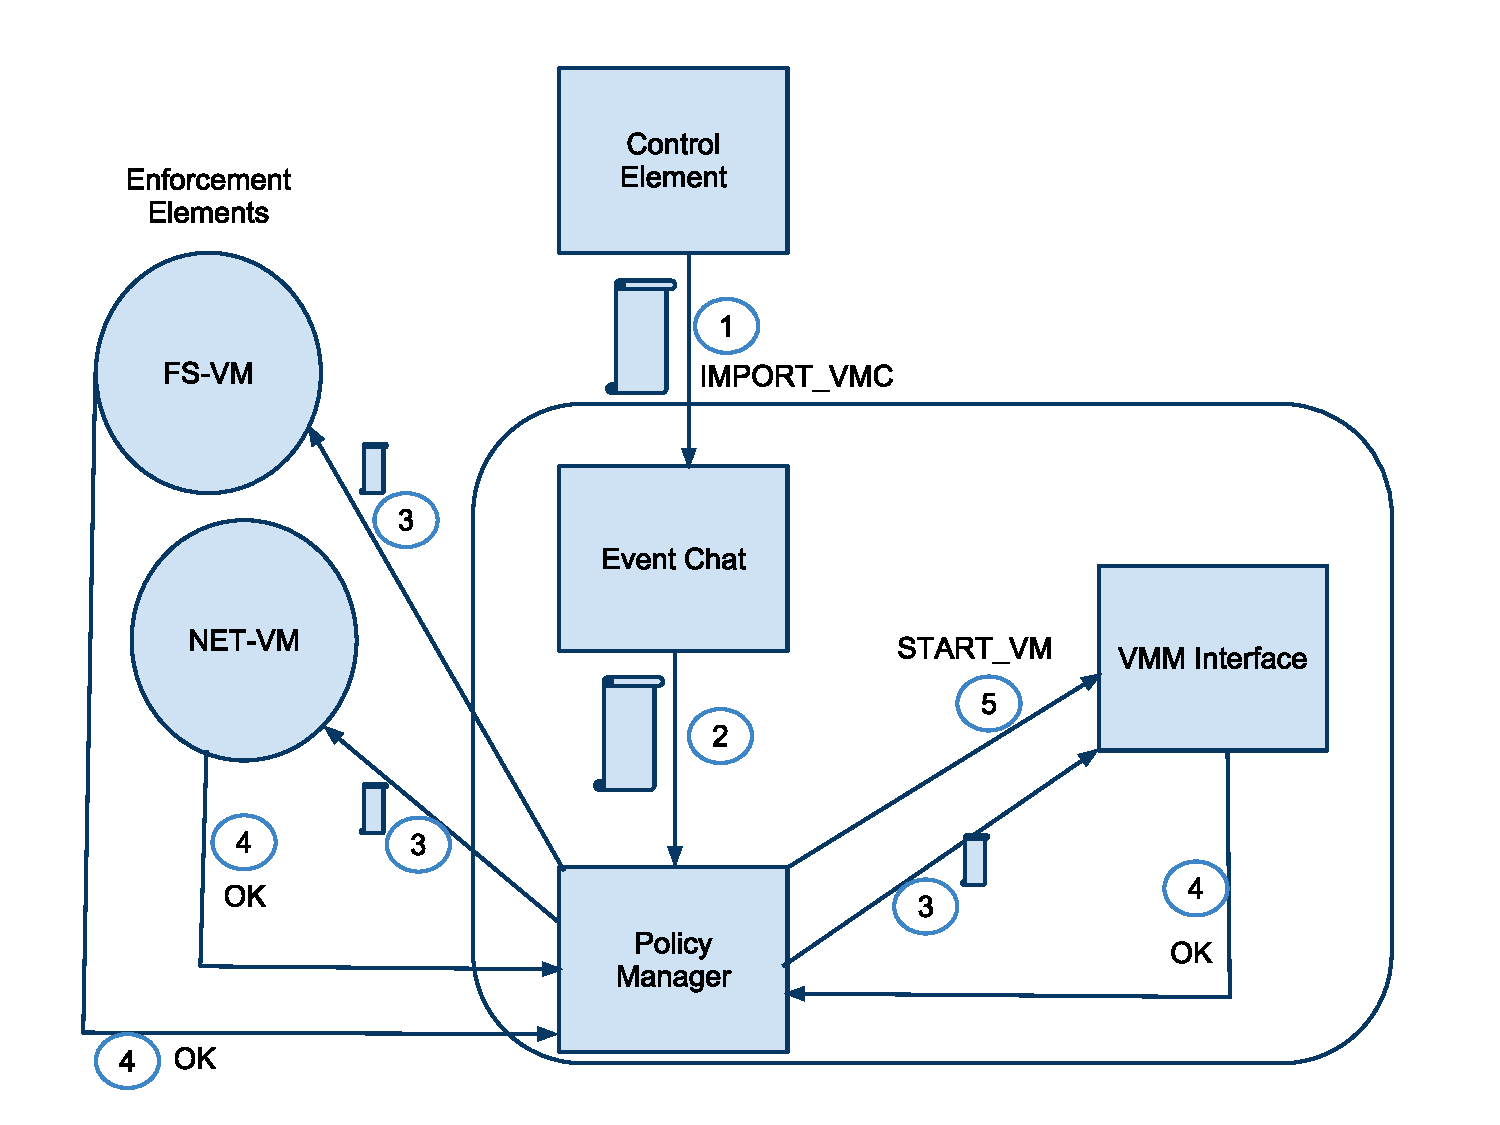
\includegraphics[scale=.7]{figs/StartVM}
\end{centering}
\end{figure}

\section{Virtual Machine Contracts}

As was described in Chapter 2 on related work, there is a fair amount of work in the virtual machine contract (VMC) space and we have been involved with much of it. VMCs are not yet significantly mature, however. Many of the important concepts have been presented \cite{virtual_machine_contract_ICAC09} and OVF is starting to be used in practice among the key virtualization players. While OVF is a step in the right direction, it still lacks many proposed features that allow us to use it directly for the Rapid Recovery Desktop system. OVF still has a long ways to go to progress from the high level theory of interchangeable VMs ~\cite{dmtf_newsletter, vmware_ovf_website, citrix_ovf_article, rhev_announce_2010} to putting that theory into practice in real world scenarios \cite {ovf_vmware_to_kvm_2010,fedora_virtAppliances, kensho_ovf_vmware_article}. 

One of the main purposes of the virtual machine contract system found in this dissertation is to bridge the gap between what is commonly deployed today and what is possible to be deployed today. Since standards and software release schedules tend to move slowly, it is helpful to have a flexible contract system, like the one proposed in this dissertation, to prototype and test new features. Our design does not prevent the conversion to or use of technologies like OVF, but instead, provides a way to test useful functionality so that it might one day be included in the OVF standard. So, until there is a standard that everyone can enjoy, we provide an implementation that can be used today. 

Figure \ref{lst:vmc_general} shows an example of the general syntax available with our contract system. We currently support two types of contracts, namely the virtual machine contract (VMC) and the Policy Manager Global contract. VMCs are for specifying the resources and constraints to place on a virtual appliance. Policy Manager Global contracts express a much different operational logic and policy than VMCs and are intended for use with the Policy Manager component of OSCKAR. 

The type attribute allows us to support new types in the future. For example, application specific contracts, such as for use with an application segregration tool like appify, which we mentioned briefly in Chapter 3. Application segregation contracts may need to be specified at a higher level of abstraction, since they might be more specific to applications, thus they may not care about the lower level details that the VMC does. The product developer for the appify contracts would then need to convert the appify contracts to VMCs and import them into OSCKAR. This abstraction might make the "appification" process more streamlined. On the other hand, virtual machine contracts might be able to be extended to support this distinction. This is an interesting area of future work.

The general format of the contract is a set of rule sets. There are any number of rule set types possible, but the ones that we currently have support for are vmm (for interacting with our VMM interface), builder (for interacting with our builder interface), FS-VM (for interacting with our FS-VM enforcement element), NET-VM (for interacting with our NET-VM enforcement element), and PolicyManager (for interacting with our PolicyManager enforcement element). The VMM and builder interfaces were described in sections \ref{sec:vmm-implementation} and \ref{sec:builder-implementation}. The NET-VM and FS-VM implementations are described in sections \ref{sec:net-vm-implementation} and \ref{sec:fs-vm-implementation} respectively. In section \ref{sec:example-appliances-implementation}, we will show specific examples of virtual appliances that use our contract system.

\begin{figure}[tbp]
\caption{General Virtual Machine Contract (VMC) Format}
\label{lst:vmc_general}

\begin{lstlisting}
<contract type="vmc" id="browser-appliance">
 <ruleset type="vmm">
  .
  .
 </ruleset>
 <ruleset type="builder">
 .
 .
 </ruleset>
 <ruleset type="other-interfaces">
 .
 .
 </ruleset>
 <ruleset type='FS-VM>
  <mounts>
   .
   .
  </mounts>
  <violations>
    .
    .
  </violations>
</ruleset>

  <ruleset type="NET-VM">
    <flows>
    .
    .
    </flows>

    <violations>
    .
    . 
   </violations>
 </ruleset>

  <ruleset type="other-enforcement-elements">
  .
  .
  </ruleset>
  <ruleset type='PolicyManager'>
    <responses event="some-event">
    </responses>
    <responses event="other-events">
    </responses>
  </ruleset>
</contract>
\end{lstlisting}
\end{figure}

As described in the VMM interface implementation (section \ref{sec:vmm-implementation}), we convert the contracts from our high level interfaces to the actual backend systems. So, our contract system builds upon the functionality of various virtualization systems, as well as any of the backend technologies used for the enforcement elements. For example, the native configuration files supported by technologies like libvirt are able to specify the hardware resource requirements, but do not necessarily support more advanced access control rules. Our contract system is used to handle these more advanced contracts to support the richer access control rules that we gain by using Samba mounts for our FS-VM and Open vSwitch access control rules for our NET-VM. Support for these types of options could be integrated into the backend technologies like libvirt, OVF, etc., but again this is an example of how our system can bridge that gap as needed. New technologies will always come along and interface designers may want to make use of them in ways that are not explicitly supported by the underlying technologies, but that shouldn't stop them from using the new technologies.

As described in Chapter 2 on related work, adding mandatory access control (MAC) to the virtualization layer, in the form of XSM\cite{xsm_xen_summit_3rd} or sVirt\cite{sVirt_website}, is complementary to our contract system. In order to support MAC policies like these, support would need to be integrated into the VMM interface and other enforcement elements. Implementing MAC rules as a new VMC rule set type and creating the proper enforcement elements could be a good area of future implementation work.

\section{FS-VM}
\label{sec:fs-vm-implementation}

The FS-VM implemented in this dissertation provides the basic functionality required to have a working Rapid Recovery Desktop system, but we believe that future development on a more advanced FS-VM is a rich area of future work. Our implementation is based on Samba, since it supports a variety of guest types, including Windows and Linux. 

Our FS-VM is able to allow specific virtual appliances to get read or read/write access to the specific mount points specified in the virtual appliance's VMC. A proof of concept implementation of read and write rate-limiting was done by parsing the log file produced by Samba's vfs\_full\_audit module, but this work has not yet been integrated into our current system. (Implementation done in previous work\cite{rapid_recovery_paper_05} was done with kernel modfications to NFS). The design of the new implementation, when integrated will not require kernel modifications. The basic idea is that when the  vfs\_full\_audit module is turned on it produces log entries for the access types configured for the shares that it is auditing. Then, the FS-VM enforcement mechanism can parse these logs and watch for violations (for example, too many reads in a given amount of time). One important feature that is currently missing in our in-progress implementation is an append-only option. Adding this functionality would require either adding features to Samba to support it, using a more advanced file system, such as the a log-structured file system (LFS)\cite{rosenblum_lfs_1992 }, with built-in support, or wrapping the file system with a layer with more advanced support, such as SELinux \cite{smalley_2001}.

An example file system rule set that allows mounting, read/write access, and rate limiting in our implementation is shown in Figure \ref{lst:fs_vm}.

\begin{figure}[tbp]
\caption{FS-VM example rule set}
\label{lst:fs_vm}

\begin{lstlisting}
<ruleset type='FS-VM>

  <mounts>
    <mount from="$FS-VM:/downloads" write="true"
       to="$HOME/downloads">
    <mount from="$FS-VM:/photos" read="true" 
       to="$HOME/photos read-rate="5 files/min">
  </mounts>

  <violations>
    <violation="read-rate-violation" 
        raise="PolicyManager.read-rate-violation $VM">
  </violations>

</ruleset>

<ruleset type='PolicyManager'>

<responses event="PolicyManager.read-rate-violation">
      <response event="PolicyManager.log_violation" 
         argument="$ARG" />
      <response event="RapidRecoveryDesktop_control.alert_user" 
         argument="$ARG" />      
      <response event="vmm.destroy_vm" argument="$ARG" />
      <response event="builder.restore_cow_vm" argument="$ARG" />
      <respons event="vmm.start_vm" argument="$ARG" />
 </responses>

</ruleset>
\end{lstlisting}
\end{figure}

In Figure \ref{lst:fs_vm}, the FS-VM rule set defines mount points, with access permissions and rate limiting options and violations, with events to raise when a violation is noticed. Note that \$ARG corresponds to the VM that the violation refers to, which is replaced on the fly by OSCKAR. For this example, we consider a browser appliance, that has write access to the downloads mount point and read access to the photos mount point (to upload to a photo site). We assume that the user is only allowed to upload a certain number of photos per minute to the server, so we impose a read limit on the number of photos that can be read. When the FS-VM detects a violation, it will send a "PolicyManager.read-rate-violation" event. The corresponding PolicyManger ruleset block tells PolicyManager the set of responses that it should take. In this example, PolicyManger will log the violation, notify our Rapid Recovery Desktop control element and then refresh the state of the VM, by restoring it to the last know good state. We will evaluate the recovery process in more detail in the evaluation section.

\section{NET-VM}
\label{sec:net-vm-implementation}

There are several approaches to virtual networking, which include a variety of software networking devices (e.g. virtual bridges or switches), combination solutions that use virtualization-aware network hardware and software virtual switches that cooperate with that hardware, and software networking devices that offload virtual networking to standard physical network hardware with standard networking techniques. The differences in the various approaches distinguish between where enforcement elements reside. For instance some network hardware vendors think that more capabilities should be pushed into the hardware. Others argue that requiring new complicated switching devices that are virtualization-aware is the wrong approach. For more details on the alternatives in general, interested readers are referred to\cite{ovs_hotnets_2009, casado_hotnets_2008, cisco_nexus_website, vepa_2008, vntag_2008, vmware_vNetwork_Distributed_Switch_website}.

For our Rapid Recovery Desktop design we would like to have the enforcement within the desktop system itself, so that we can enforce policy without requiring users to buy extra hardware. The Open vSwitch software, which is the latest in open source virtual switch technology allows us to have that control. So, our NET-VM component is based on Open vSwitch and then it is integrated into our architecture. We choose this approach for our specific situation, since it allows us to apply access control at the virtual network layer. Similar proprietary approaches exist in commercial products~\cite{vmware_vNetwork_Distributed_Switch_website, cisco_nexus_website}. Another reason that we choose Open vSwitch is that it supports external management of vswitches. This will allow us to run a controller in a dedicated NET-VM component that can manage all of the vswitches. Thus, allowing us to continue to separate mechanism and policy. More details of Open vSwitch and the technologies that are possible to integrate with it will be discussed in the future work section of Chapter 6. For now, we note that we use its built-in switch controller technology, but plan to implement a proper controller (using a technology like NOX\cite{nox_website}) in the future.

The access control rules that we can apply to the virtual switches allow us to allow only the flows specified in the virtual appliance contract. For instance, for a browser appliance, we can allow only dns lookups and outgoing web connections HTTP (port 80) and HTTPS (port 443). An example of the flow language needed to limit this access is shown in Figure \ref{lst:net_vm}. The NET-VM rule set includes a set of flows that allow for outgoing web, dns, and dhcp traffic. All other traffic is not allowed to flow over the virtual switch.

\begin{figure}[tbp]
\caption{NET-VM example rule set}
\label{lst:net_vm}

\begin{lstlisting}
<ruleset type="NET-VM">

<flows>
  <flow action="allow" type="web" direction="outgoing" />
  <flow action="allow" type="dns" direction="outgoing" />
  <flow action="allow" type="dhcp" direction="outgoing" />
</flows>

</ruleset>
\end{lstlisting}
\end{figure}

If desired, we could also apply network rate limiting for virtual appliances using built-in Open vSwitch functionality. Open vSwitch keeps aggregate packet count and size of packets for each flow. So, obtaining the rate of flow is straight-forward. Using this information, we could act on virtual appliance contract rules that specify expected network rate limits. We have not yet implemented network rate limiting, but it would be a good future implementation work.  An example NET-VM rule set that provides rate-limiting and response is shown in Figure \ref{lst:net_vm-rate}.

\begin{figure}[tbp]
\caption{Rate-limiting NET-VM example rule set}
\label{lst:net_vm-rate}

\begin{lstlisting}
<ruleset type="NET-VM">
<flows>
  <flow action="allow" type="web" direction="outgoing" 
     rate="1Mbit/s"/>
  <flow action="allow" type="dns" direction="outgoing" 
     rate="10 lookups per second" />
  <flow action="allow" type="dhcp" direction="outgoing" 
     rate="2 requests per day"/>
</flows>
  <violations>
    <violation="web-rate-violation" 
       raise="PolicyManager.web-rate-violation $VM">
    <violation="dns-rate-violation" 
       raise="PolicyManager.dns-rate-violation $VM">
    <violation="dhcp-rate-violation" 
       raise="PolicyManager.dhcp-rate-violation $VM">
    <violation="invalid-outgoing-port-request" 
       raise="PolicyManager.invalid-outgoing-port-request $VM">
  </violations>
</ruleset>
<ruleset type='PolicyManager'>
<responses event="PolicyManager.web-rate-violation">
      <response event="PolicyManager.log_violation" 
         argument="$ARG" />
 </responses>
<responses event="PolicyManager.dns-rate-violation">
      <response event="PolicyManager.log_violation" 
         argument="$ARG" />
      <response event="RapidRecoveryDesktop_control.alert_user" 
         argument="$ARG" />      
      <response event="vmm.destroy_vm" 
         argument="$ARG" />
      <response event="builder.restore_cow_vm" 
         argument="$ARG" />
      <respons event="vmm.start_vm" 
         argument="$ARG" />
 </responses>
<responses event="PolicyManager.dhcp-rate-violation">
      <response event="PolicyManager.log_violation" 
         argument="$ARG" />
      <response event="RapidRecoveryDesktop_control.alert_user" 
         argument="$ARG" />      
 </responses>
<responses event="PolicyManager.invalid-outgoing-port-request">
      <response event="PolicyManager.log_violation" argument="$ARG" />
      <response event="RapidRecoveryDesktop_control.alert_user" 
          argument="$ARG" />      
      <response event="vmm.destroy_vm" argument="$ARG" />
      <response event="builder.restore_cow_vm" argument="$ARG" />
      <respons event="vmm.start_vm" argument="$ARG" />
 </responses>
</ruleset>
\end{lstlisting}
\end{figure}

The NET-VM rule sets in Figure \ref{lst:net_vm-rate} add rate-limiting rules and a set of violations. Each of the violations raises an event to Policy Manager. Policy Manager in turn takes various responses. We may consider web traffic rate violation to be not too severe and we only log it. A DNS violation might be considered more severe, however, and we want to stop the VM and restore it to a known good state. For a DHCP violation, it might be helpful to notify the user or an administrator. Some discussion of how we respond in various cases is discussed in more detail in Chapter 5 on evaluation. 

Another set of violations that we can handle are invalid outgoing port requests. When a VM attempts to create a flow that is not in its allowed list, it is disallowed automatically by Open vSwitch, since an explicit allow rule is not in place. This type of situation might signal a problem with the VM. So one possible response could be to restore the VM to a known good state.

Finer granularity of control is also possible for any of the enforcement elements. The enforcement element designer needs only to add the functionality and make it known. For the NET-VM, some possible enhancement could include allowing for some number of invalid port requests before restoring the VM, only restoring the VM some maximum number of times before simply shutting it down and alerting an administrator, or logging invalid incoming port requests for security research purposes. These options are currently not available in our NET-VM implementation, but could be added as future implementation work.

\section{Example Virtual Appliances}
\label{sec:example-appliances-implementation}

To complete our implementation of the Rapid Recovery Desktop system, we create a sample virtual appliances and its associated VMC that uses our FS-VM and NET-VM rules to specify its data and network access needs. Specifically, we create a browser virtual appliance. We present its basic implementation in this section and evaluate the effectiveness and performance of the our Rapid Recovery Desktop system as a whole in the next chapter.

\subsection{Browser Virtual Appliance}

A VMC for our example browser virtual appliance is shown in Figures \ref{lst:browser-appliance}, \ref{lst:browser-appliance-cont}, and \ref{lst:browser-appliance-cont2}. We collect together the various components from previous sections of the chapter into one cohesive contract that protects our browser virtual appliance. This appliance is introduced to the system by our Rapid Recovery Desktop control element. This control element calls OSCKAR library methods to import the contract and start the virtual appliance. 

\begin{figure}[tbp]
\caption{Browser Appliance Virtual Machine Contract (VMC) (1 of 3)}
\label{lst:browser-appliance}

\begin{lstlisting}
<contract type="vmc" id="browser-appliance">
 <ruleset type="vmm">
    <name>browser</name>
    <memory>
      <min>128MB</min>
      <max>1G</max>
      <default>512MB</default>
    </memory>
    <disks>
      <cowdisk type="qcow2" cowbase="browser.qcow2">browser</cowdisk>
    </disks>
    <vnics>
      <vnic type="bridge" />
    </vnics>
    <graphics>
      <graphic type="vnc" />
    </graphics>
    <displays>  
      <display type='vga' />
    </displays>
    <features>
      <feature>acpi</feature>
    </features>
  </ruleset>
 <ruleset type="builder">
   <os type="linux" flavor="ubuntu" version="9.10" />
   <disk type="disk" size="10240" sparse="true" format="qcow2">browser.qcow2
   </disk>
   <partitions>
     <partition filesystem="ext3" mountpoint="/" size="10G" bootable="true">1
     </partition>
   </partitions>
   <users>
     <user logindisabled="true">root</user>
     <user password="ubuntu" groups="ubuntu,admin">ubuntu</user>
   </users>
   <packages>
     <package name="openssh-server" action="add" />
     <package name="sl" action="add" />    
   </packages>
   <installmirror>http://mirror.clarkson.edu/ubuntu</installmirror> 
  </ruleset>
\end{lstlisting}
\end{figure}

\begin{figure}[tbp]
\caption{Browser Appliance Virtual Machine Contract (VMC) Continued (2 of 3)}
\label{lst:browser-appliance-cont}

\begin{lstlisting}
<ruleset type='FS-VM>
  <mounts>
    <mount from="$FS-VM:/downloads" write="true" 
       to="$HOME/downloads">
    <mount from="$FS-VM:/photos" read="true" 
      to="$HOME/photos read-rate="5 files/min">
  </mounts>
  <violations>
    <violation="read-rate-violation" 
       raise="PolicyManager.read-rate-violation $VM">
  </violations>
</ruleset>
<ruleset type="NET-VM">
<flows>
  <flow action="allow" type="web" direction="outgoing" 
     rate="1Mbit/s"/>
  <flow action="allow" type="dns" direction="outgoing" 
     rate="10 lookups per second" />
  <flow action="allow" type="dhcp" direction="outgoing" 
     rate="2 requests per day"/>
</flows>
  <violations>
    <violation="web-rate-violation" 
       raise="PolicyManager.web-rate-violation $VM">
    <violation="dns-rate-violation" 
       raise="PolicyManager.dns-rate-violation $VM">
    <violation="dhcp-rate-violation" 
       raise="PolicyManager.dhcp-rate-violation $VM">
    <violation="invalid-outgoing-port-request" 
       raise="PolicyManager.invalid-outgoing-port-request $VM">
  </violations>
</ruleset>
\end{lstlisting}
\end{figure}

\begin{figure}[tbp]
\caption{Browser Appliance Virtual Machine Contract (VMC) Continued (3 of 3)}
\label{lst:browser-appliance-cont2}

\begin{lstlisting}
<ruleset type='PolicyManager'>
<responses event="PolicyManager.read-rate-violation">
      <response event="PolicyManager.log_violation" 
         argument="$ARG" />
      <response event="RapidRecoveryDesktop_control.alert_user"
         argument="$ARG" />      
      <response event="vmm.destroy_vm" argument="$ARG" />
      <response event="builder.restore_cow_vm" argument="$ARG" />
      <respons event="vmm.start_vm" argument="$ARG" />
 </responses>
<responses event="PolicyManager.web-rate-violation">
      <response event="PolicyManager.log_violation" argument="$ARG" />
 </responses>
<responses event="PolicyManager.dns-rate-violation">
      <response event="PolicyManager.log_violation" argument="$ARG" />
      <response event="RapidRecoveryDesktop_control.alert_user" 
         argument="$ARG" />      
      <response event="vmm.destroy_vm" argument="$ARG" />
      <response event="builder.restore_cow_vm" argument="$ARG" />
      <respons event="vmm.start_vm" argument="$ARG" />
 </responses>
<responses event="PolicyManager.dhcp-rate-violation">
      <response event="PolicyManager.log_violation" argument="$ARG" />
      <response event="RapidRecoveryDesktop_control.alert_user" 
         argument="$ARG" />      
 </responses>
<responses event="PolicyManager.invalid-outgoing-port-request">
      <response event="PolicyManager.log_violation" argument="$ARG" />
      <response event="RapidRecoveryDesktop_control.alert_user" 
         argument="$ARG" />      
      <response event="vmm.destroy_vm" argument="$ARG" />
      <response event="builder.restore_cow_vm" argument="$ARG" />
      <respons event="vmm.start_vm" argument="$ARG" />
 </responses>
</ruleset>
</contract>
\end{lstlisting}
\end{figure}

\subsection{Other Virtual Appliance Examples}

An email client virtual appliance would be similar to a browser appliance, in that it needs access to both FS-VM mount points and also NET-VM flows. The difference is that the FS-VM mount points a specific to email. For example, instead of write access to a downloads folder, write access to a mail folder would be needed instead. Read access to photos and other documents to be used as attachments may also be desired. The network flows that would be necessary are an outgoing (in the sense that the email virtual appliance connects out to the mail server) POP or IMAP flow (to receive mail) and an outgoing SMTP flow (to send mail).

Other applications that don't need any network access, such as many games and other personal-only programs, such as a diary application, would not have any NET-VM rules. They could use FS-VM rules in order to store and share data. For example they may want to have special mounts points that keep game state or journal entries. Thus, backups to the FS-VM can be made and the virtual appliances can be upgraded or rolled back as needed without losing the user's personal data.

Server virtual appliances, such as a web server appliance would have incoming net flows added to their NET-VM rule sets. They would not have any outgoing rule sets, so that if an attacker compromised the web server, it would not be able to download malware to the web server appliance. The web appliance would also want FS-VM mounts for its web content directory and may also want to mount the server logs to the FS-VM in order to keep visitor traffic information protected over a period of time, even if the web server itself needs to be rolled back to a known good state due to upgrade failures or being compromised.

Finally, financial virtual appliances, which were discussed in detail in Chapter 3 on design, could be implemented in various ways depending on the details needs of the user and specific application.

We've now shown the complete implementation of the Rapid Recovery Desktop system. In the next chapter we evaluate its performance, effectiveness, and recovery properties.

